\documentclass[aspectratio=169,10pt,fontset=none]{ctexbeamer}

\usetheme{Madrid}
\usecolortheme{seahorse}
\usefonttheme{professionalfonts}

\usepackage{graphicx}
\usepackage{booktabs}
\usepackage{tabularx}
\usepackage{array}
\usepackage{tikz}
\usepackage{xcolor}
\usepackage{xurl}
\usepackage{hyperref}
\usetikzlibrary{positioning,arrows.meta}
\hypersetup{unicode=true}

\setCJKmainfont[BoldFont={WenQuanYi Zen Hei}]{WenQuanYi Micro Hei}
\setCJKsansfont[BoldFont={WenQuanYi Zen Hei}]{WenQuanYi Micro Hei}
\setCJKmonofont{WenQuanYi Micro Hei Mono}
\setmainfont{DejaVu Sans}
\setsansfont{DejaVu Sans}
\graphicspath{{figures/}}
\urlstyle{tt}

\definecolor{FlyBlue}{HTML}{275A9A}
\definecolor{FlyGreen}{HTML}{2D7554}
\definecolor{FlyOrange}{HTML}{B9652B}
\definecolor{FlyRed}{HTML}{9B2C2C}
\definecolor{FlyGray}{HTML}{F5F7FA}
\definecolor{FlyDark}{HTML}{1F2933}

\setbeamercolor{title}{fg=white,bg=FlyBlue}
\setbeamercolor{frametitle}{fg=white,bg=FlyBlue}
\setbeamercolor{structure}{fg=FlyBlue}
\setbeamercolor{block title}{fg=white,bg=FlyBlue}
\setbeamercolor{block body}{fg=FlyDark,bg=FlyGray}
\setbeamercolor{alerted text}{fg=FlyRed}
\setbeamertemplate{navigation symbols}{}
\setbeamertemplate{headline}{}
\setbeamerfont{footline}{family=\sffamily,size=\scriptsize}
\setbeamertemplate{footline}{%
  \leavevmode%
  \hbox{%
    \begin{beamercolorbox}[wd=\paperwidth,ht=2.3ex,dp=1ex,right]{author in head/foot}%
      \normalfont\sffamily\scriptsize\insertframenumber{} / \inserttotalframenumber\hspace{1.5ex}%
    \end{beamercolorbox}%
  }%
}

\newcommand{\blue}[1]{\textcolor{FlyBlue}{\textbf{#1}}}
\newcommand{\green}[1]{\textcolor{FlyGreen}{\textbf{#1}}}
\newcommand{\orange}[1]{\textcolor{FlyOrange}{\textbf{#1}}}
\newcommand{\red}[1]{\textcolor{FlyRed}{\textbf{#1}}}
\newcommand{\smallnote}[1]{\vspace{0.25em}{\scriptsize\textcolor{FlyDark}{#1}}}

\title[赛博果蝇组会汇报]{赛博果蝇能否把左右脑递质侧化变成可验证的记忆假说？}
\subtitle{FlyWire 结构发现、连接组传播、DPM 光遗传预测与 OCT/MCH 行为验证}
\author{bio\_fly 项目组会汇报}
\institute{\url{/unify/ydchen/unidit/bio_fly}}
\date{}

\begin{document}

\begin{frame}
  \titlepage
  \vspace{-0.8em}
  \begin{block}{今天的主线}
    我们不是只展示一个果蝇动画，而是回答一个具体问题：\orange{右侧血清素富集、左侧谷氨酸偏置}这种蘑菇体输入侧化，能否通过连接组传播到记忆相关读出，并转化成湿实验可检验的 DPM 光遗传和 OCT/MCH 行为预测？
  \end{block}
\end{frame}

\begin{frame}{先给结论}
\small
\begin{columns}[T,onlytextwidth]
  \begin{column}{0.48\textwidth}
    \begin{block}{当前最稳的发现}
      \begin{itemize}
        \item KC 输入存在稳定递质侧化。
        \item \orange{5-HT/Serotonin 右偏}：11/11 KC 类型同向。
        \item \blue{Glu/Glutamate 左偏}：7/11 KC 类型同向且显著。
        \item 最强区域是 $\alpha'\beta'$，与记忆巩固相关。
      \end{itemize}
    \end{block}
  \end{column}
  \begin{column}{0.48\textwidth}
    \begin{block}{仿真给出的推进}
      \begin{itemize}
        \item 侧化 seed 能传播到 memory axis、DAN、APL、DPM、MBON/MBIN。
        \item DPM 光遗传预测优先测试 617/627 nm 红光协议。
        \item OCT/MCH 中 weak OCT / strong MCH conflict 是最敏感行为条件。
        \item MB 侧化扰动行为层尚未显著，这是重要风险。
      \end{itemize}
    \end{block}
  \end{column}
\end{columns}
\vspace{0.2em}
\begin{center}
\blue{一句话：结构侧化已经很强，功能传播有支持，真实行为因果还需要湿实验闭环。}
\end{center}
\end{frame}

\begin{frame}{必要名词：非生物背景也能跟上}
\scriptsize
\begin{tabularx}{\textwidth}{@{}p{2.7cm}X@{}}
\toprule
\textbf{名词} & \textbf{本汇报中的含义} \\
\midrule
MB / 蘑菇体 & 果蝇学习和记忆核心脑区，尤其与气味记忆相关。\\
KC & Kenyon cell，蘑菇体主要细胞，接收气味和调节输入。\\
5-HT / Ser & 血清素，调节性神经递质；本项目发现 KC 输入中右侧更强。\\
Glu & 谷氨酸；本项目发现 KC 输入中多数左侧更强。\\
DAN / MBON & 多巴胺教学信号 / 蘑菇体输出信号，参与奖励、惩罚和行为选择。\\
APL / DPM & 蘑菇体反馈和记忆维持相关神经元；DPM 是本轮光遗传验证重点。\\
CS+ / CS- & 训练中与奖励或惩罚配对的气味 / 对照或竞争气味。\\
OCT / MCH & 3-octanol / 4-methylcyclohexanol，两种经典果蝇气味。\\
LI & Laterality index，$(R-L)/(R+L)$；正值偏右，负值偏左。\\
\bottomrule
\end{tabularx}
\end{frame}

\begin{frame}{研究设计：从结构发现到可验证预测}
\small
\centering
\begin{tikzpicture}[
  node distance=0.55cm,
  box/.style={draw=FlyBlue, thick, rounded corners=2pt, fill=FlyGray, align=center, minimum width=2.35cm, minimum height=0.92cm},
  arrow/.style={-{Latex[length=2mm]}, thick, FlyBlue}
]
\node[box] (data) {FlyWire v783\\连接组 + NT 预测};
\node[box, right=of data] (seed) {选择侧化 seed\\右 5-HT / 左 Glu KC};
\node[box, right=of seed] (prop) {GPU signed\\multi-hop propagation};
\node[box, right=of prop] (readout) {memory axis\\DAN/APL/DPM/MBON};
\node[box, below=0.9cm of prop] (validation) {DPM 光遗传\\OCT/MCH 行为预测};
\draw[arrow] (data) -- (seed);
\draw[arrow] (seed) -- (prop);
\draw[arrow] (prop) -- (readout);
\draw[arrow] (readout) |- (validation);
\end{tikzpicture}
\vspace{0.8em}
\begin{block}{关键点}
这里的“赛博果蝇”是公开可审计的替代接口：连接组传播 + 透明行为代理。它不是 Eon 私有闭环系统的逐参数复刻。
\end{block}
\end{frame}

\begin{frame}{数据和实验条件}
\small
\begin{columns}[T,onlytextwidth]
  \begin{column}{0.48\textwidth}
    \begin{block}{结构与传播数据}
      \begin{itemize}
        \item FlyWire adult brain：约 13.9 万神经元。
        \item signed connectivity：约 1509 万条边。
        \item 目标群：KC、MBON、DAN、APL、DPM、DN。
        \item 传播设置：3 hop，max active 5000，GPU sparse propagation。
      \end{itemize}
    \end{block}
  \end{column}
  \begin{column}{0.48\textwidth}
    \begin{block}{行为和验证条件}
      \begin{itemize}
        \item OCT/MCH mirror-side：CS+ 左右平衡，避免位置偏置。
        \item 关键行为指标：choice index、approach margin、early turning。
        \item DPM 协议扫描：opsin、波长、频率、脉宽、时长、光强。
        \item 湿实验对照：no-opsin、red-light-only、retinal-minus、180 度旋转。
      \end{itemize}
    \end{block}
  \end{column}
\end{columns}
\end{frame}

\begin{frame}{结果 1：KC 输入存在递质侧化}
\scriptsize
\begin{columns}[T,onlytextwidth]
  \begin{column}{0.59\textwidth}
    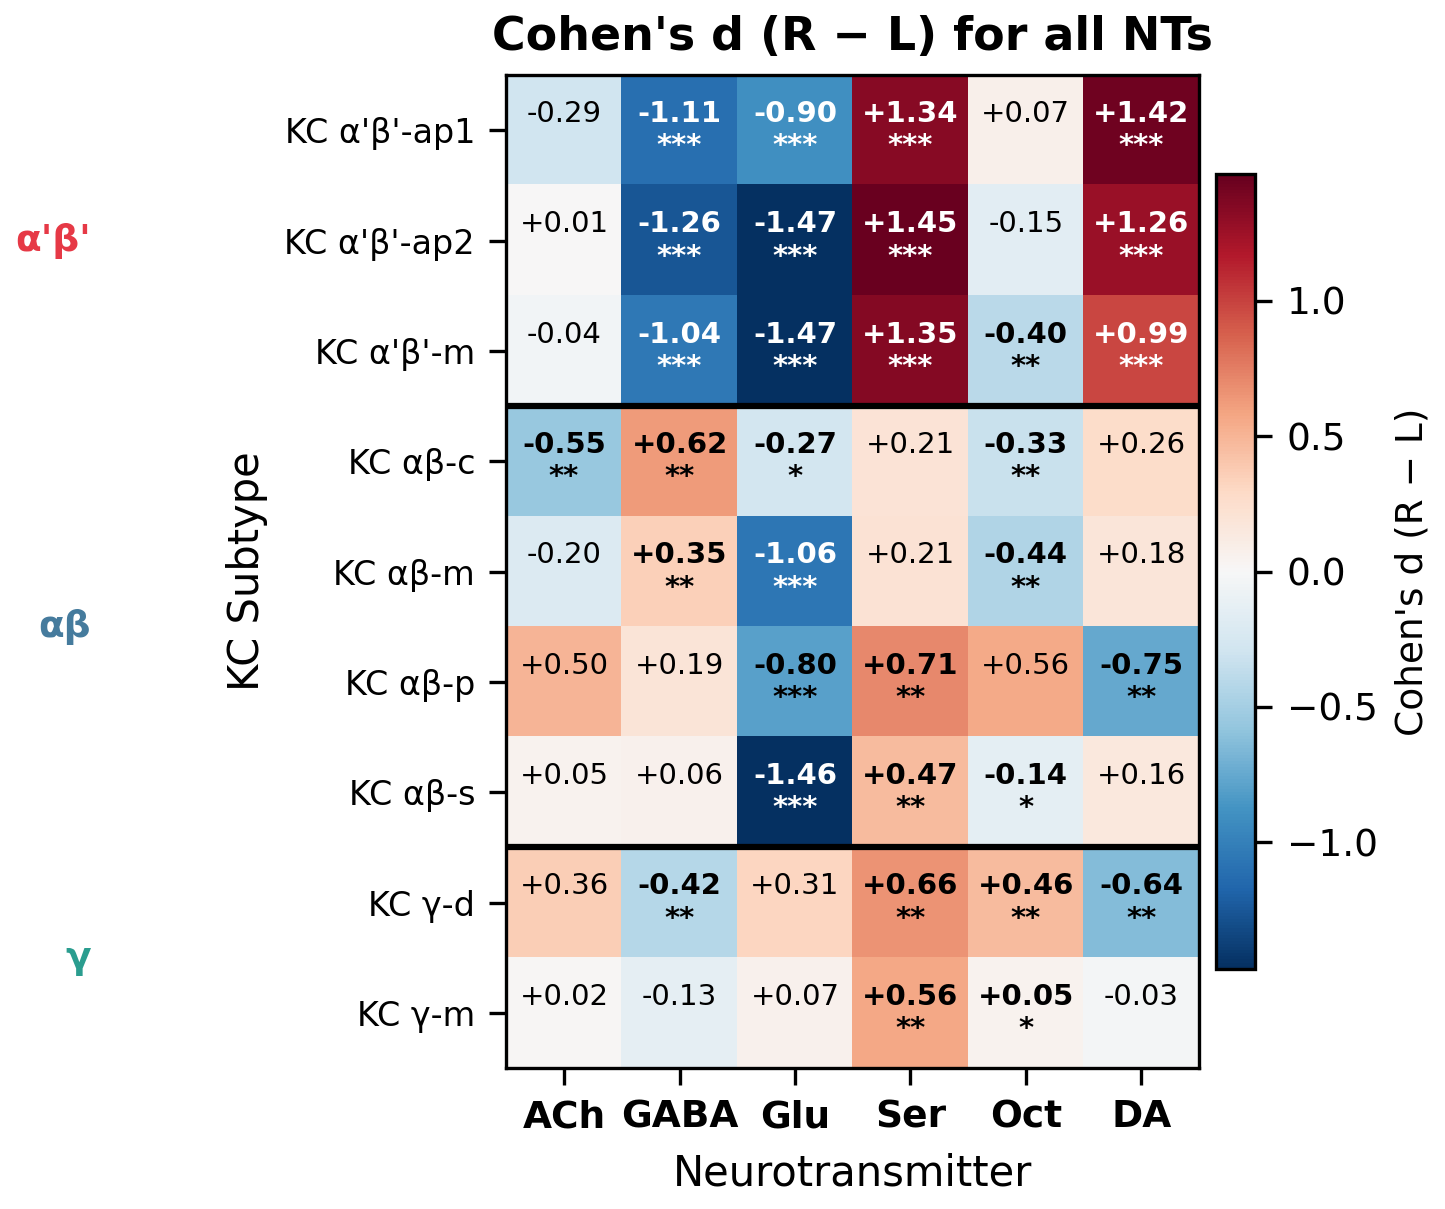
\includegraphics[width=0.96\textwidth]{Fig_ext1_cohens_d_heatmap_all_NT.png}
  \end{column}
  \begin{column}{0.37\textwidth}
    \begin{block}{怎么看}
      红色表示右侧更高，蓝色表示左侧更高；行是 KC 亚型，列是递质。
    \end{block}
    \begin{block}{读出的结论}
      \begin{itemize}
        \item 5-HT 基本整列右偏。
        \item Glu 多数左偏。
        \item $\alpha'\beta'$ 区效应最大。
        \item KC 输出仍主要是 ACh，所以这是输入侧化。
      \end{itemize}
    \end{block}
  \end{column}
\end{columns}
\end{frame}

\begin{frame}{结果 2：侧化 seed 不是随机 KC 的等价替代}
\scriptsize
\begin{columns}[T,onlytextwidth]
  \begin{column}{0.58\textwidth}
    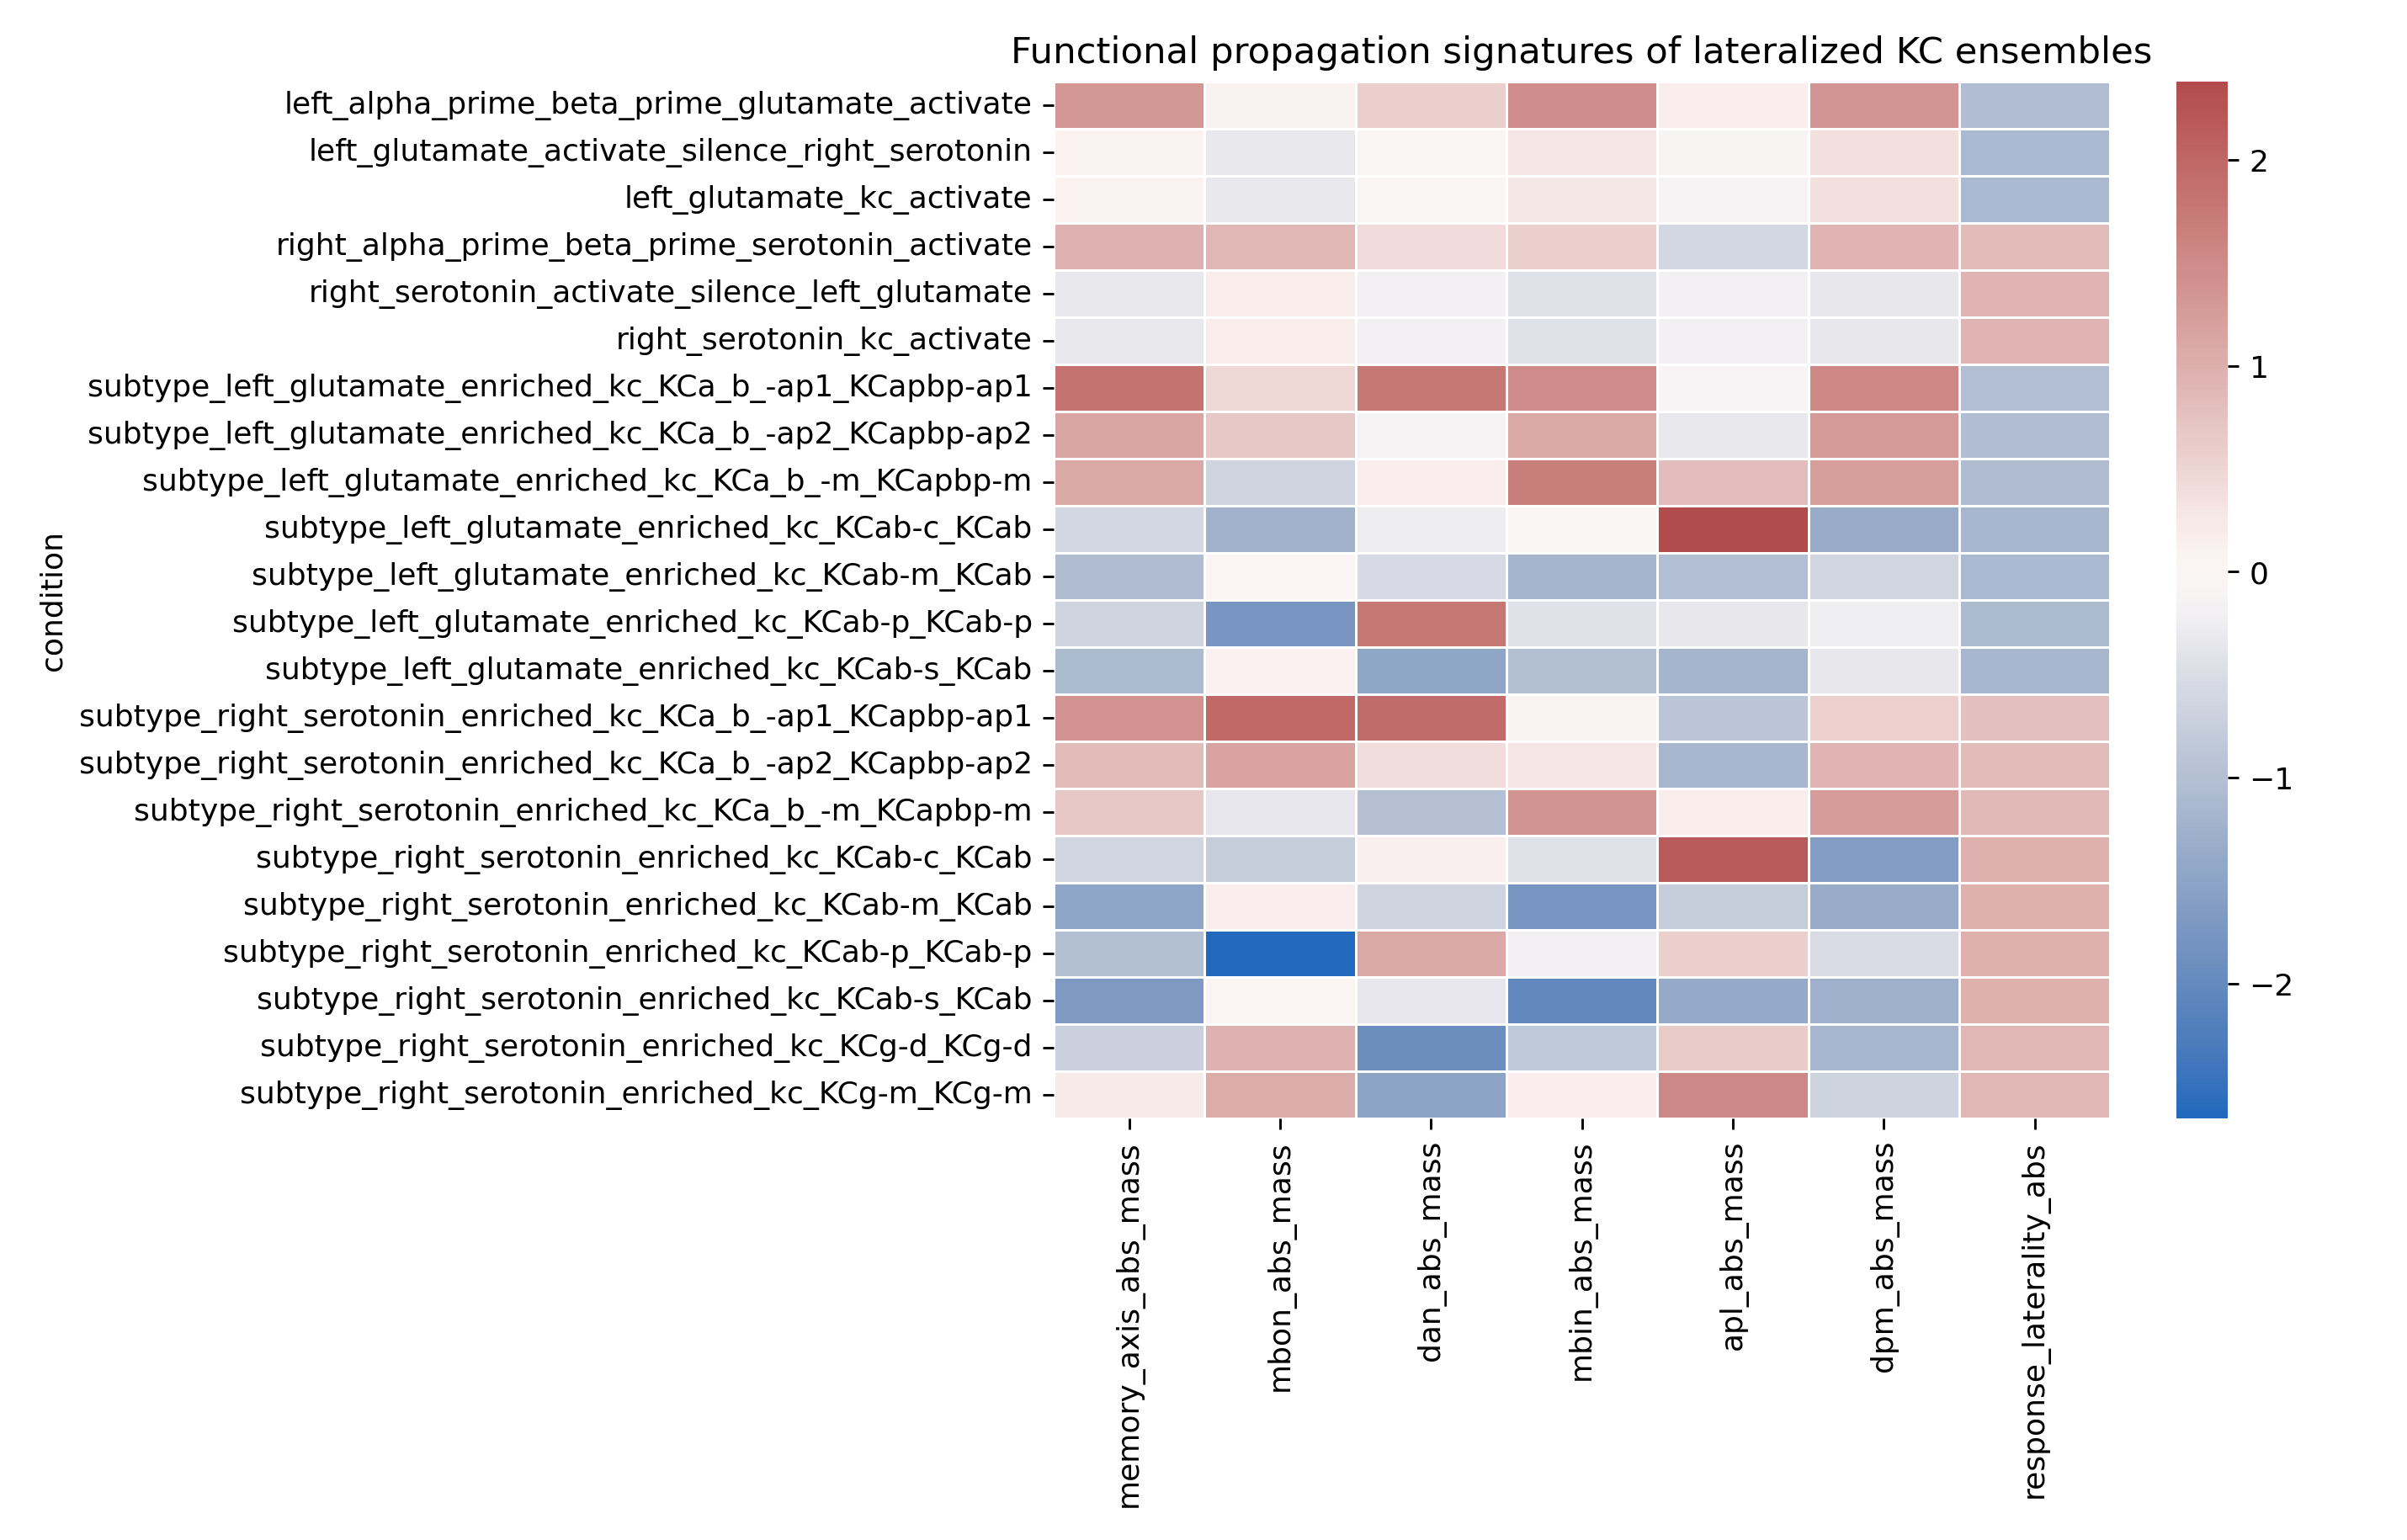
\includegraphics[width=\textwidth]{Fig2_functional_metric_heatmap.png}
  \end{column}
  \begin{column}{0.38\textwidth}
    \begin{block}{实验方法}
      选择右侧 5-HT-rich KC 和左侧 Glu-rich KC 作为 seed，在 FlyWire signed graph 上传播，并与同侧同规模随机 KC 对照比较。
    \end{block}
    \begin{block}{主要结果}
      \begin{itemize}
        \item 右 5-HT seed 改变 DAN、APL、DPM、左右读出。
        \item 左 Glu seed 更广泛影响 memory axis、MBON/MBIN、DAN、DPM。
        \item 最强结果 FDR $q=0.038$。
      \end{itemize}
    \end{block}
  \end{column}
\end{columns}
\end{frame}

\begin{frame}{结果 3：MB 结构侧化能到达 DN 出口}
\scriptsize
\begin{columns}[T,onlytextwidth]
  \begin{column}{0.50\textwidth}
    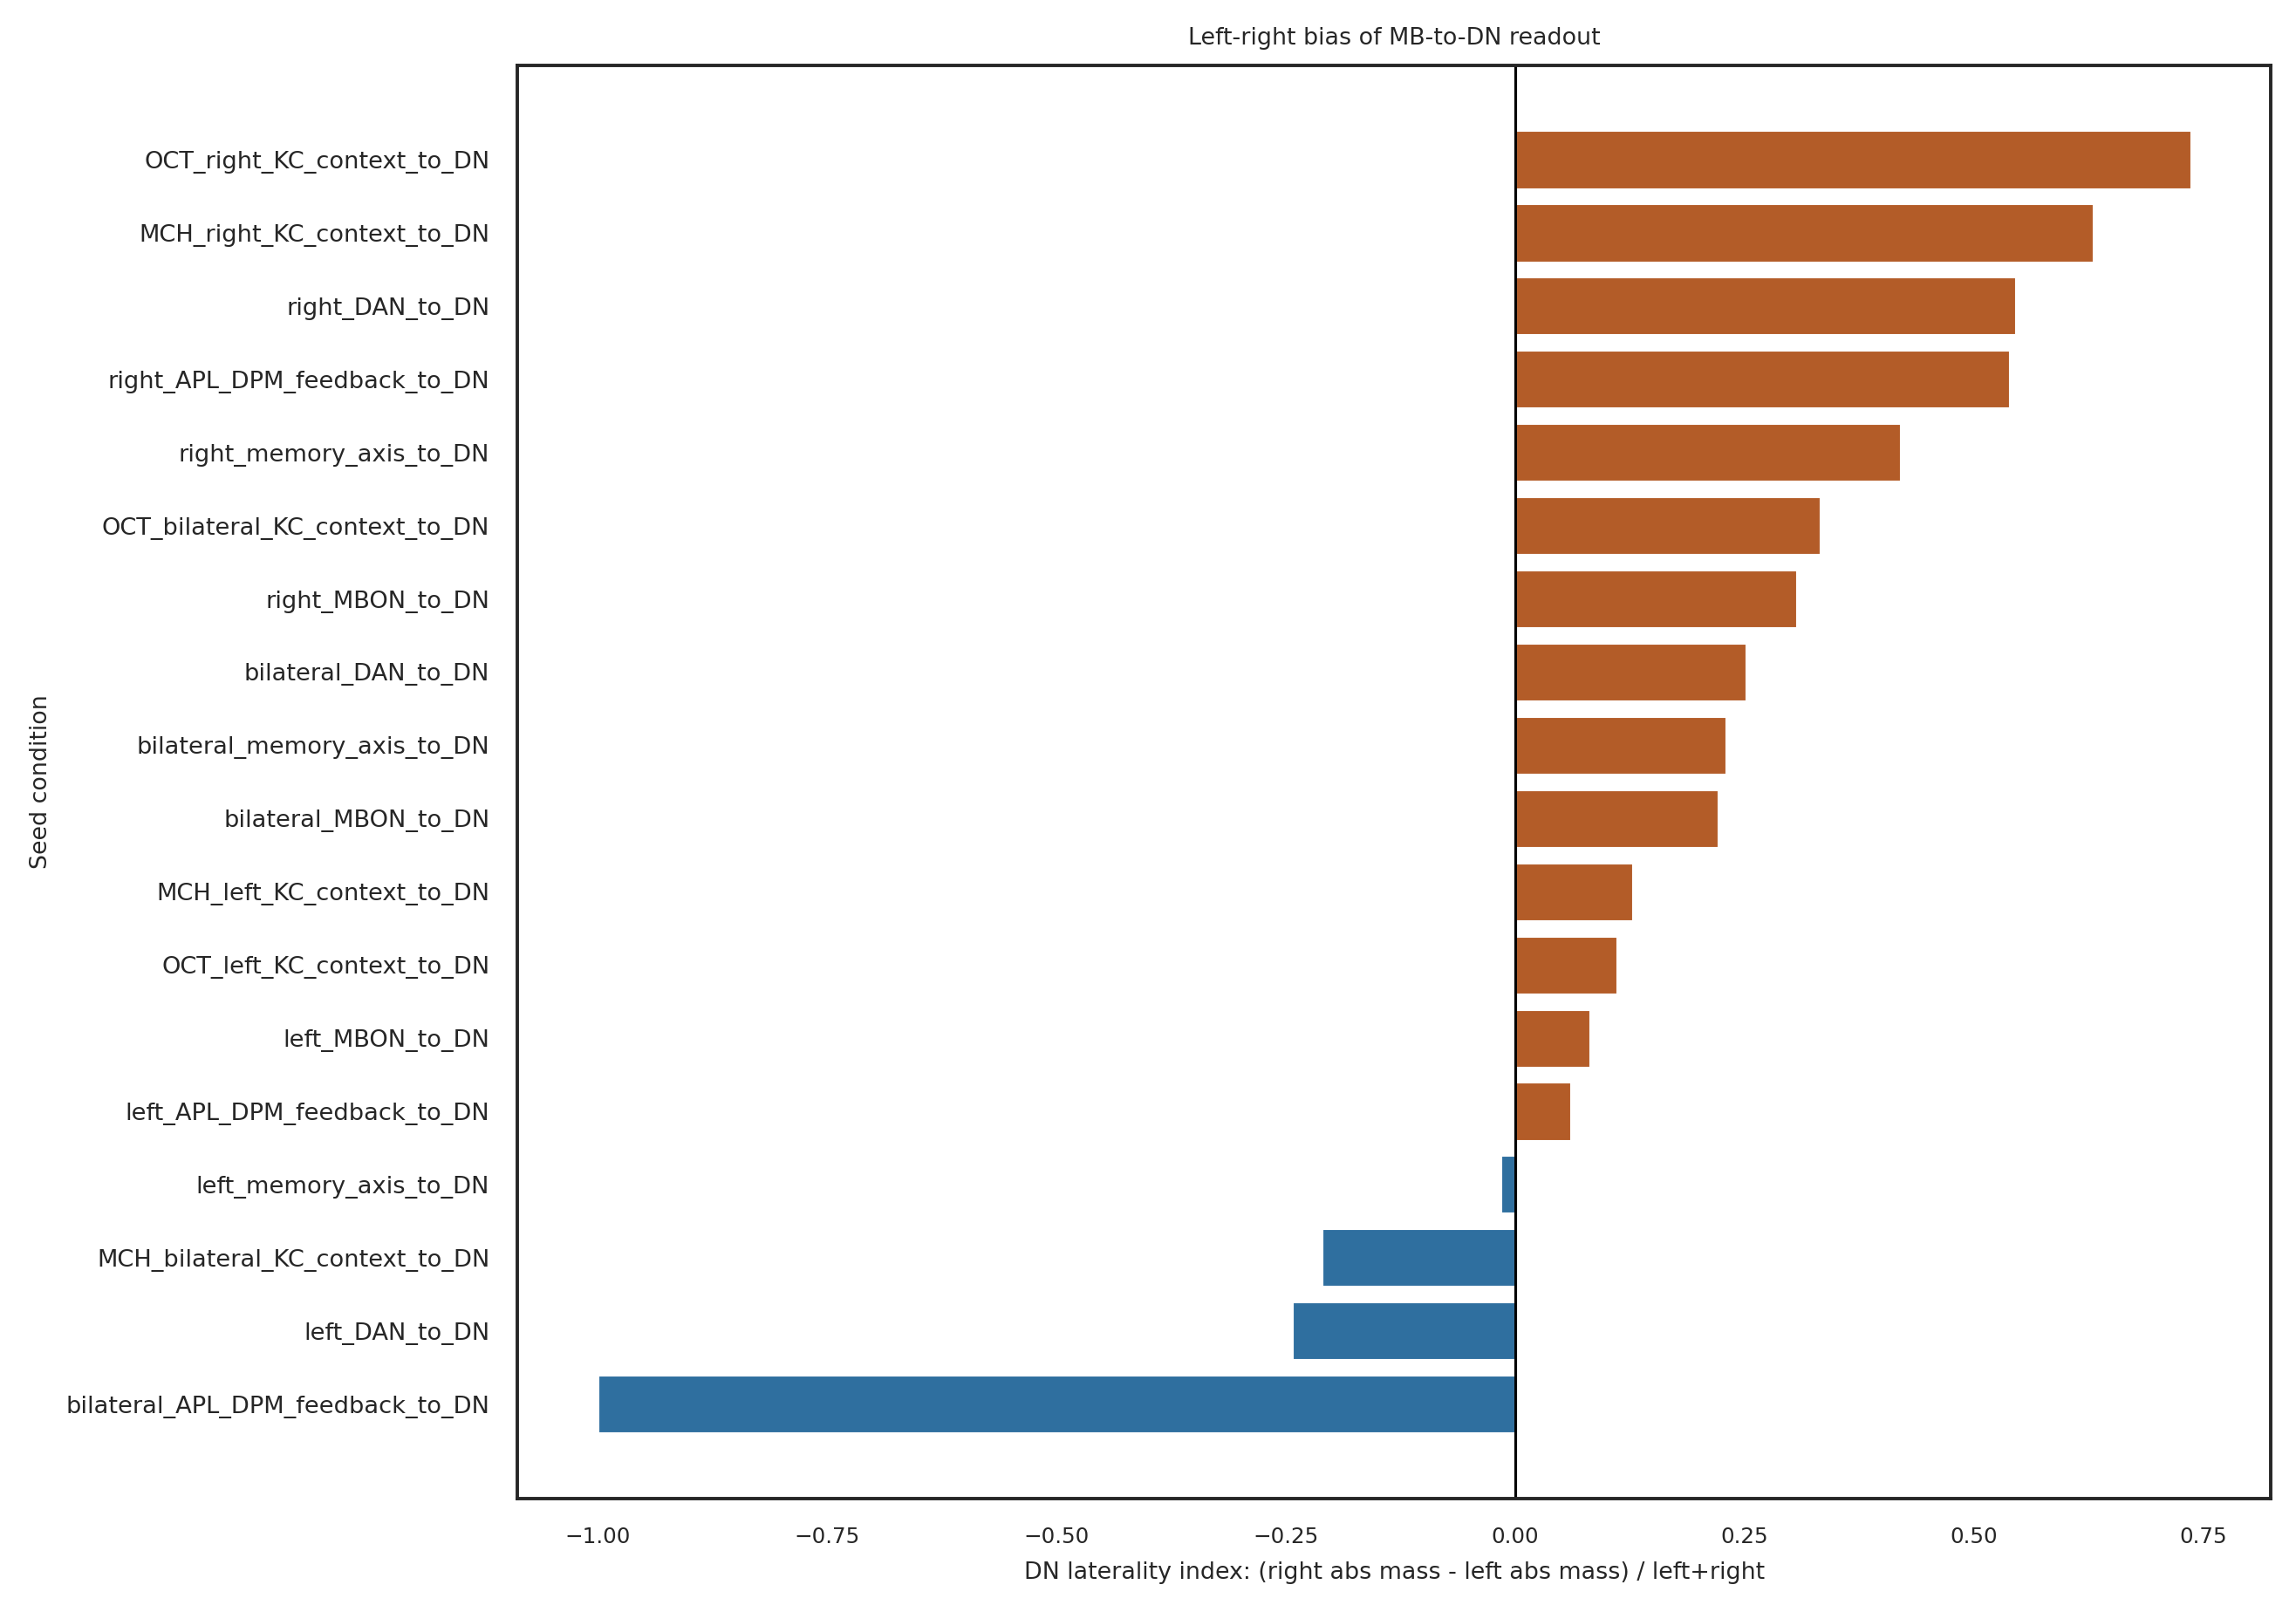
\includegraphics[width=\textwidth]{Fig_mb_dn_laterality_index.png}
  \end{column}
  \begin{column}{0.46\textwidth}
    \begin{tabular}{@{}lrrr@{}}
    \toprule
    \textbf{条件} & \textbf{DN数} & \textbf{abs mass} & \textbf{LI}\\
    \midrule
    left MBON & 202 & 0.0648 & +0.082\\
    right MBON & 149 & 0.0341 & +0.307\\
    bilateral memory axis & 108 & 0.0245 & +0.230\\
    right memory axis & 110 & 0.0215 & +0.420\\
    left memory axis & 111 & 0.0215 & -0.016\\
    \bottomrule
    \end{tabular}
    \vspace{0.55em}
    \begin{block}{解释}
      left MBON 的总响应更强；right MBON/right memory axis 的右偏更明显。强度和左右偏向是两个不同维度。
    \end{block}
  \end{column}
\end{columns}
\end{frame}

\begin{frame}{赛博果蝇接口：为什么要加 DN / motor bridge}
\small
\begin{columns}[T,onlytextwidth]
  \begin{column}{0.58\textwidth}
    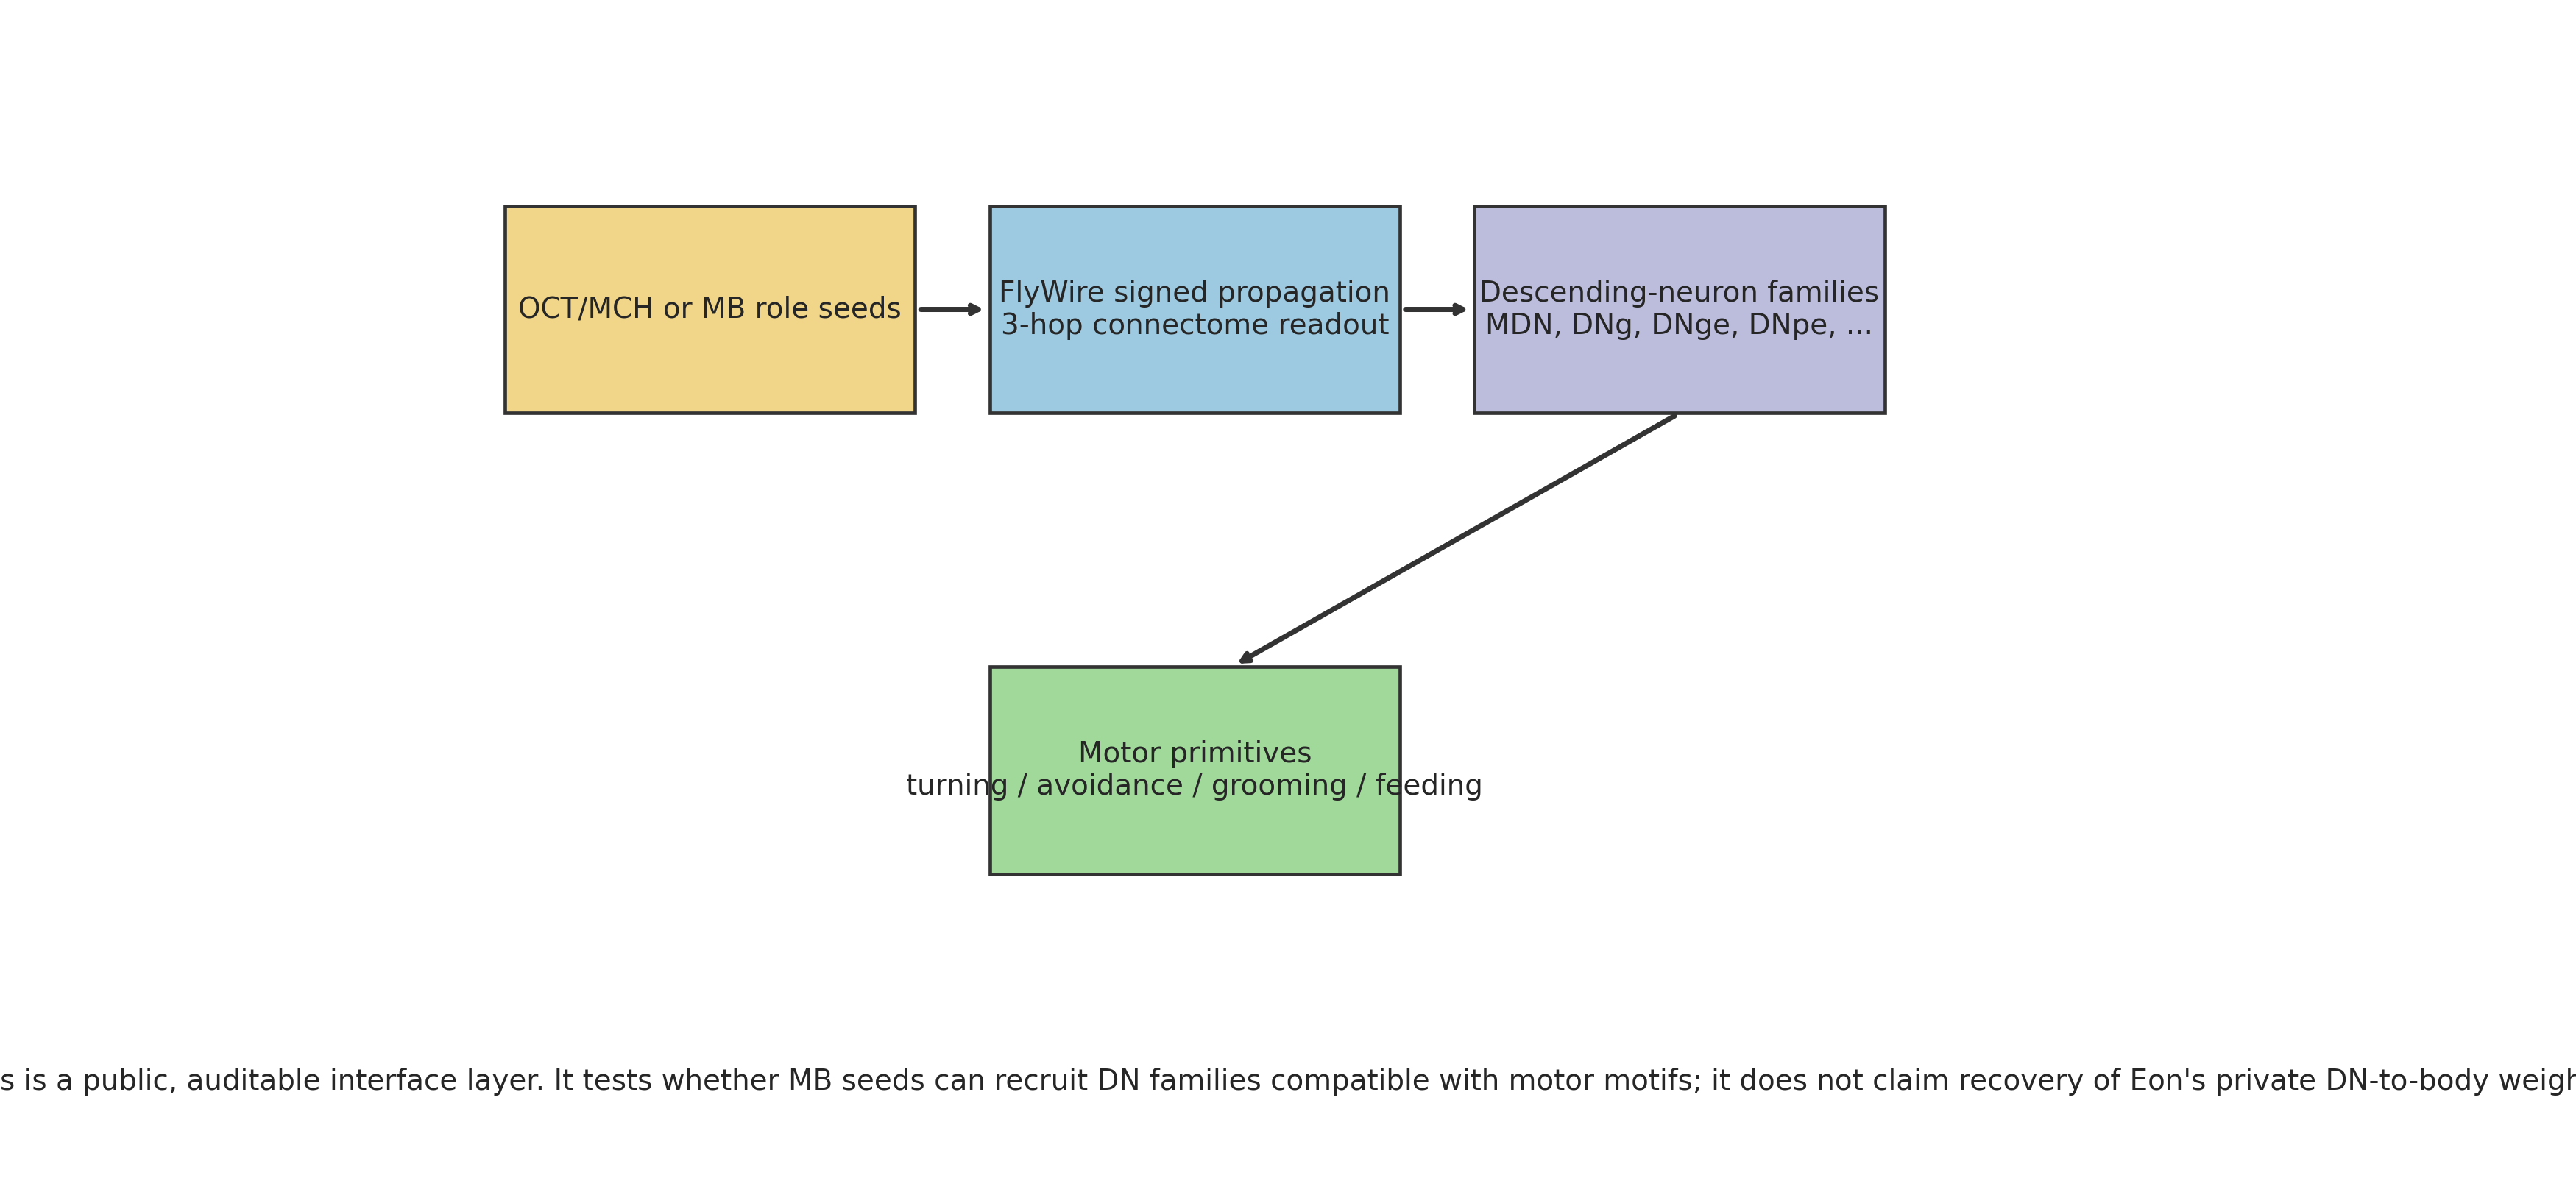
\includegraphics[width=\textwidth]{Fig_mb_dn_motor_mechanism.png}
  \end{column}
  \begin{column}{0.38\textwidth}
    \begin{block}{公开资料缺口}
      Eon 没有公开完整 DN-to-body 权重和闭环控制参数。
    \end{block}
    \begin{block}{我们的替代做法}
      把系统拆成可审计层级：MB seed $\to$ DN family $\to$ motor primitive $\to$ OCT/MCH 行为代理。
    \end{block}
    \begin{alertblock}{严谨边界}
      这可以产生实验预测，但不能说已经复刻 Eon 私有数字果蝇。
    \end{alertblock}
  \end{column}
\end{columns}
\end{frame}

\begin{frame}{结果 4：DPM 光遗传协议预测}
\scriptsize
\begin{columns}[T,onlytextwidth]
  \begin{column}{0.55\textwidth}
    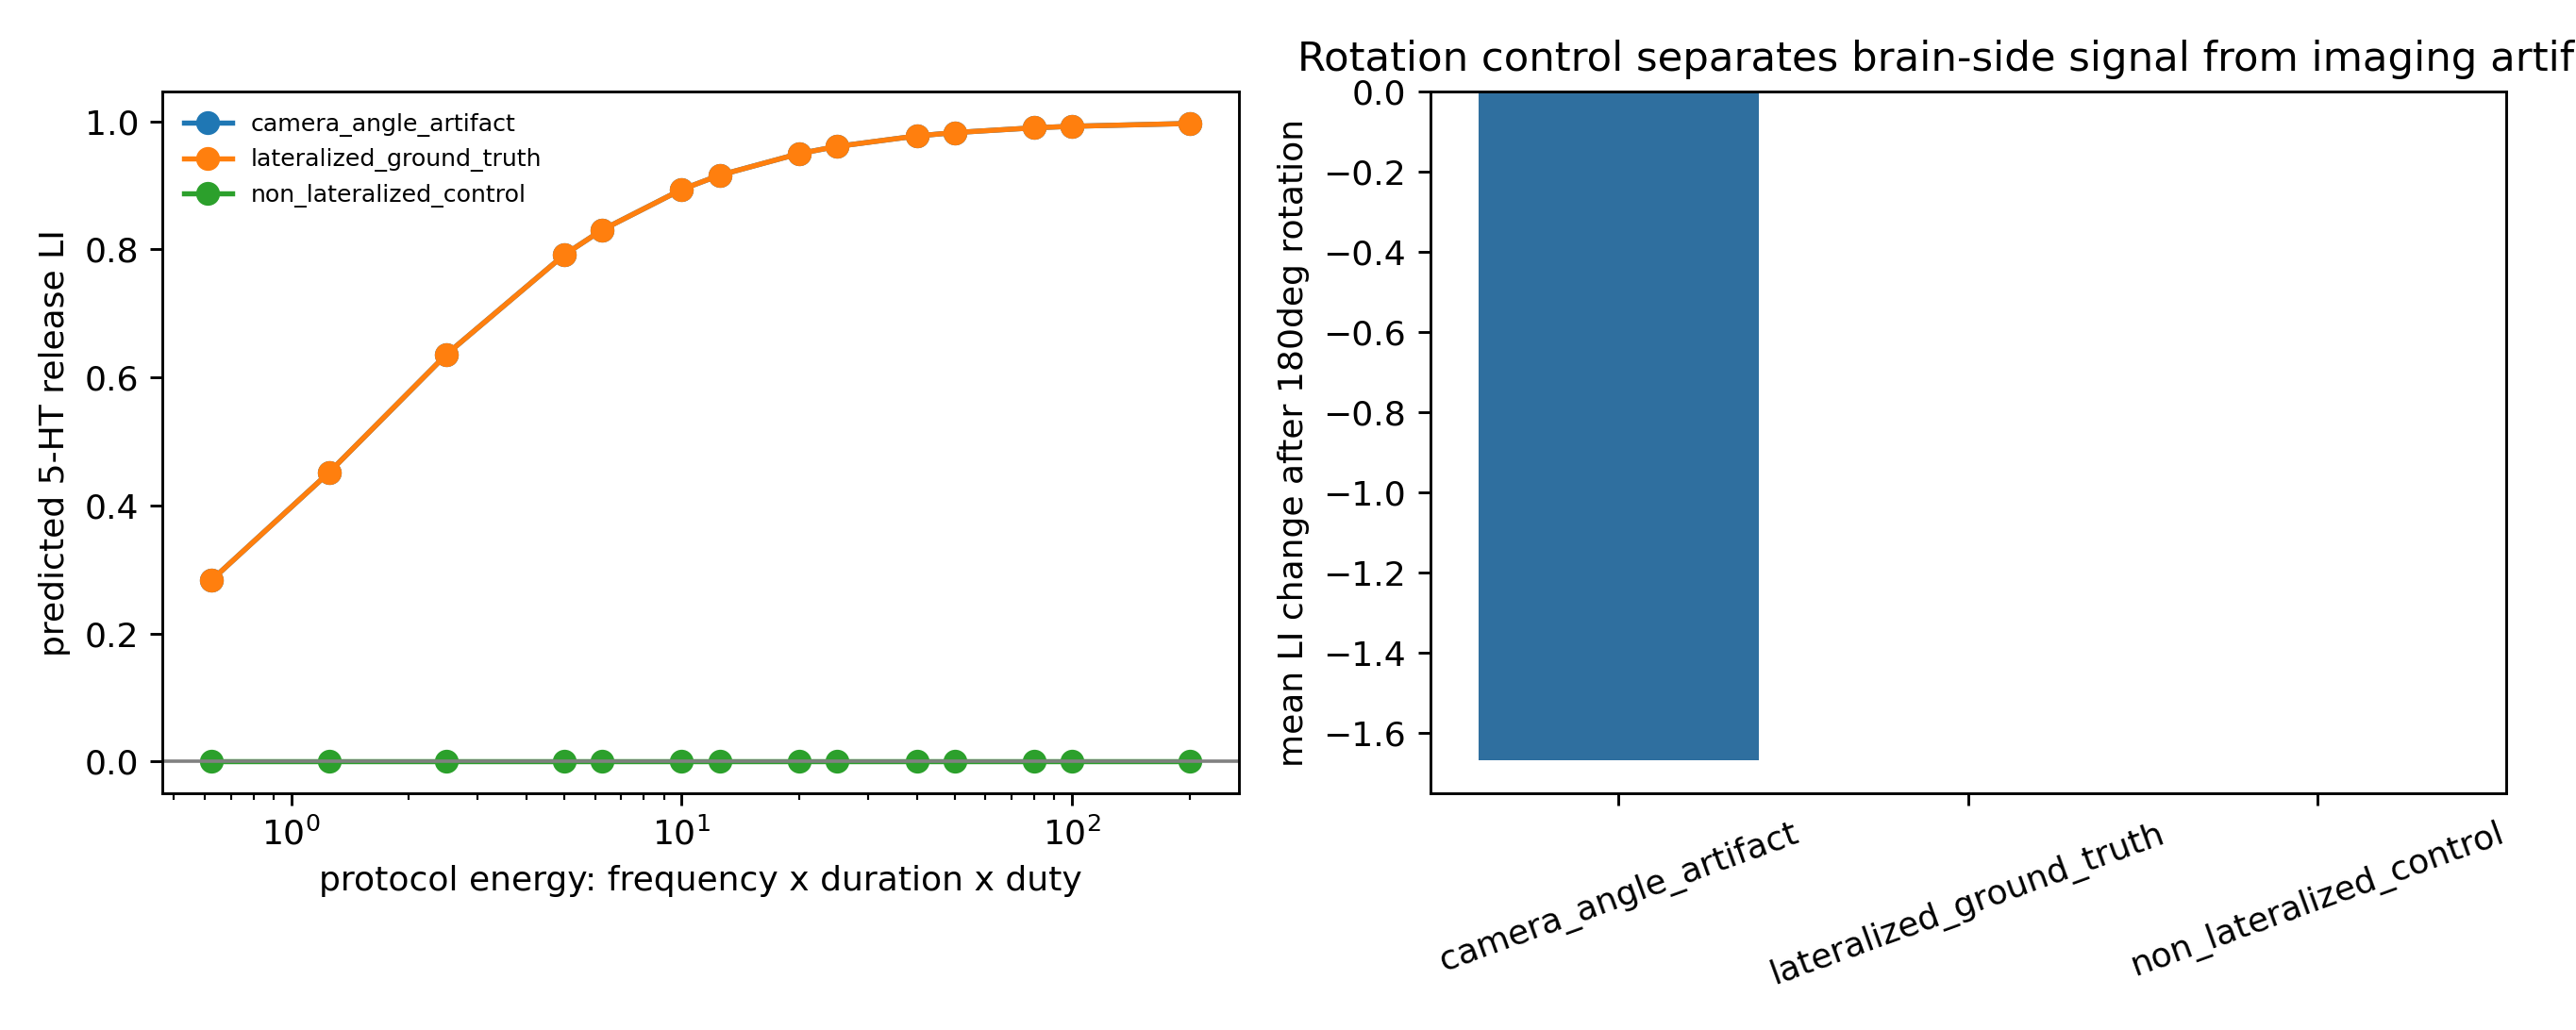
\includegraphics[width=\textwidth]{Fig_dpm_optogenetic_protocol_predictions.png}
  \end{column}
  \begin{column}{0.41\textwidth}
    \begin{block}{仿真实验}
      以 DPM neuron 为 seed，扫描 CsChrimson、ReaChR、ChR2 的波长、频率、脉宽、时长和光强。
    \end{block}
    \begin{block}{推荐湿实验起点}
      \begin{itemize}
        \item CsChrimson：617 nm。
        \item ReaChR：627 nm。
        \item 40 Hz，20 ms pulse，5 s train。
        \item 低到中等光强起步。
      \end{itemize}
    \end{block}
  \end{column}
\end{columns}
\end{frame}

\begin{frame}{结果 5：DPM 激活后的 release pattern 预测}
\scriptsize
\begin{columns}[T,onlytextwidth]
  \begin{column}{0.55\textwidth}
    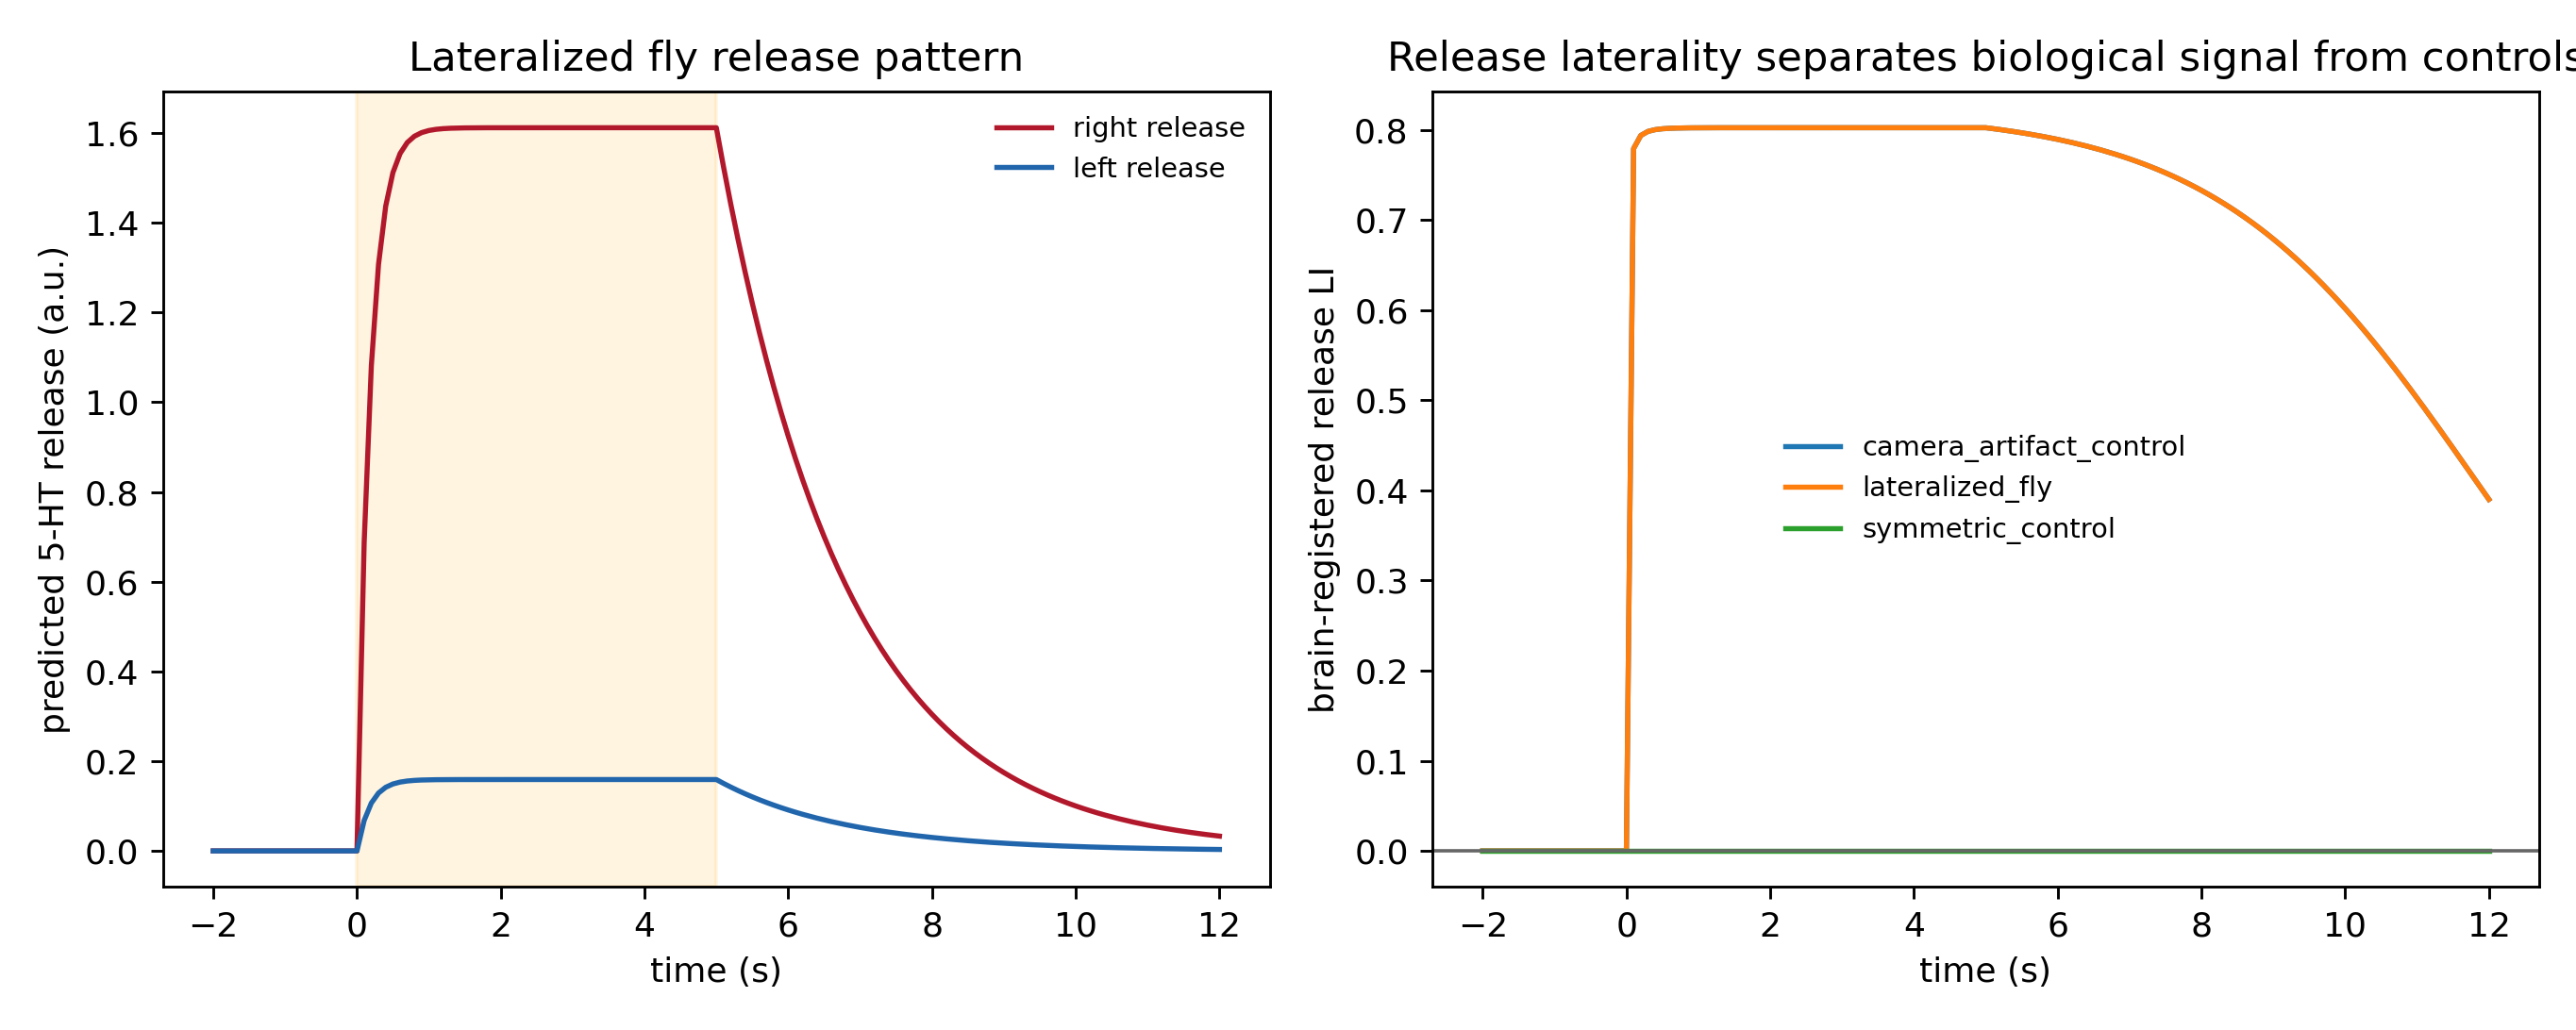
\includegraphics[width=\textwidth]{Fig_dpm_5ht_release_timecourses.png}
  \end{column}
  \begin{column}{0.41\textwidth}
    \begin{block}{预测}
      DPM 红光激活后，按脑侧注册的 5-HT/KC readout 保持右偏，top protocol 的 peak release LI 约 0.80。
    \end{block}
    \begin{block}{关键控制}
      同一成像设置做 180 度水平旋转。若是真脑侧偏侧化，脑侧坐标 LI 不翻转；若是相机角度伪影，图像坐标 LI 会翻转。
    \end{block}
  \end{column}
\end{columns}
\end{frame}

\begin{frame}{结果 6：OCT/MCH 行为实验设计}
\small
\begin{columns}[T,onlytextwidth]
  \begin{column}{0.50\textwidth}
    \begin{block}{核心条件}
      \begin{itemize}
        \item OCT + sucrose：奖励，预期接近 OCT。
        \item MCH + sucrose：气味身份反平衡。
        \item OCT + shock：惩罚，预期回避 OCT。
        \item weak OCT / strong MCH：弱记忆和强感觉冲突。
      \end{itemize}
    \end{block}
  \end{column}
  \begin{column}{0.46\textwidth}
    \begin{block}{统计设置}
      \begin{itemize}
        \item 正式条件 n=100。
        \item CS+ 左右各半，做 mirror-side。
        \item 读出 choice index、approach margin、early turning。
        \item 多重比较使用 FDR。
      \end{itemize}
    \end{block}
  \end{column}
\end{columns}
\vspace{0.2em}
\begin{center}
\blue{weak OCT / strong MCH conflict 最适合检测 DPM/5-HT 轴的小幅行为调节。}
\end{center}
\end{frame}

\begin{frame}{结果 7：OCT/MCH 行为代理方向稳定}
\scriptsize
\begin{columns}[T,onlytextwidth]
  \begin{column}{0.55\textwidth}
    
\includegraphics[width=\textwidth]{Fig_oct_mch_formal_suite.png}
  \end{column}
  \begin{column}{0.41\textwidth}
    \begin{tabular}{@{}lcc@{}}
    \toprule
    \textbf{条件} & \textbf{选择率} & \textbf{FDR q}\\
    \midrule
    OCT+sucrose & 0.86 & $9.5{\times}10^{-14}$\\
    MCH+sucrose & 0.85 & $4.8{\times}10^{-13}$\\
    OCT+shock & 0.86 & $9.5{\times}10^{-14}$\\
    conflict & 0.88 & $3.8{\times}10^{-15}$\\
    \bottomrule
    \end{tabular}
    \vspace{0.6em}
    \begin{block}{能说明什么}
      行为代理能稳定表达奖励趋近、惩罚回避和冲突条件下的记忆驱动选择。
    \end{block}
    \begin{alertblock}{不能说明什么}
      这还不是 MB 侧化扰动的真实行为因果证据。
    \end{alertblock}
  \end{column}
\end{columns}
\end{frame}

\begin{frame}{视频展示：让实验场景可读}
\small
\begin{columns}[T,onlytextwidth]
  \begin{column}{0.63\textwidth}
    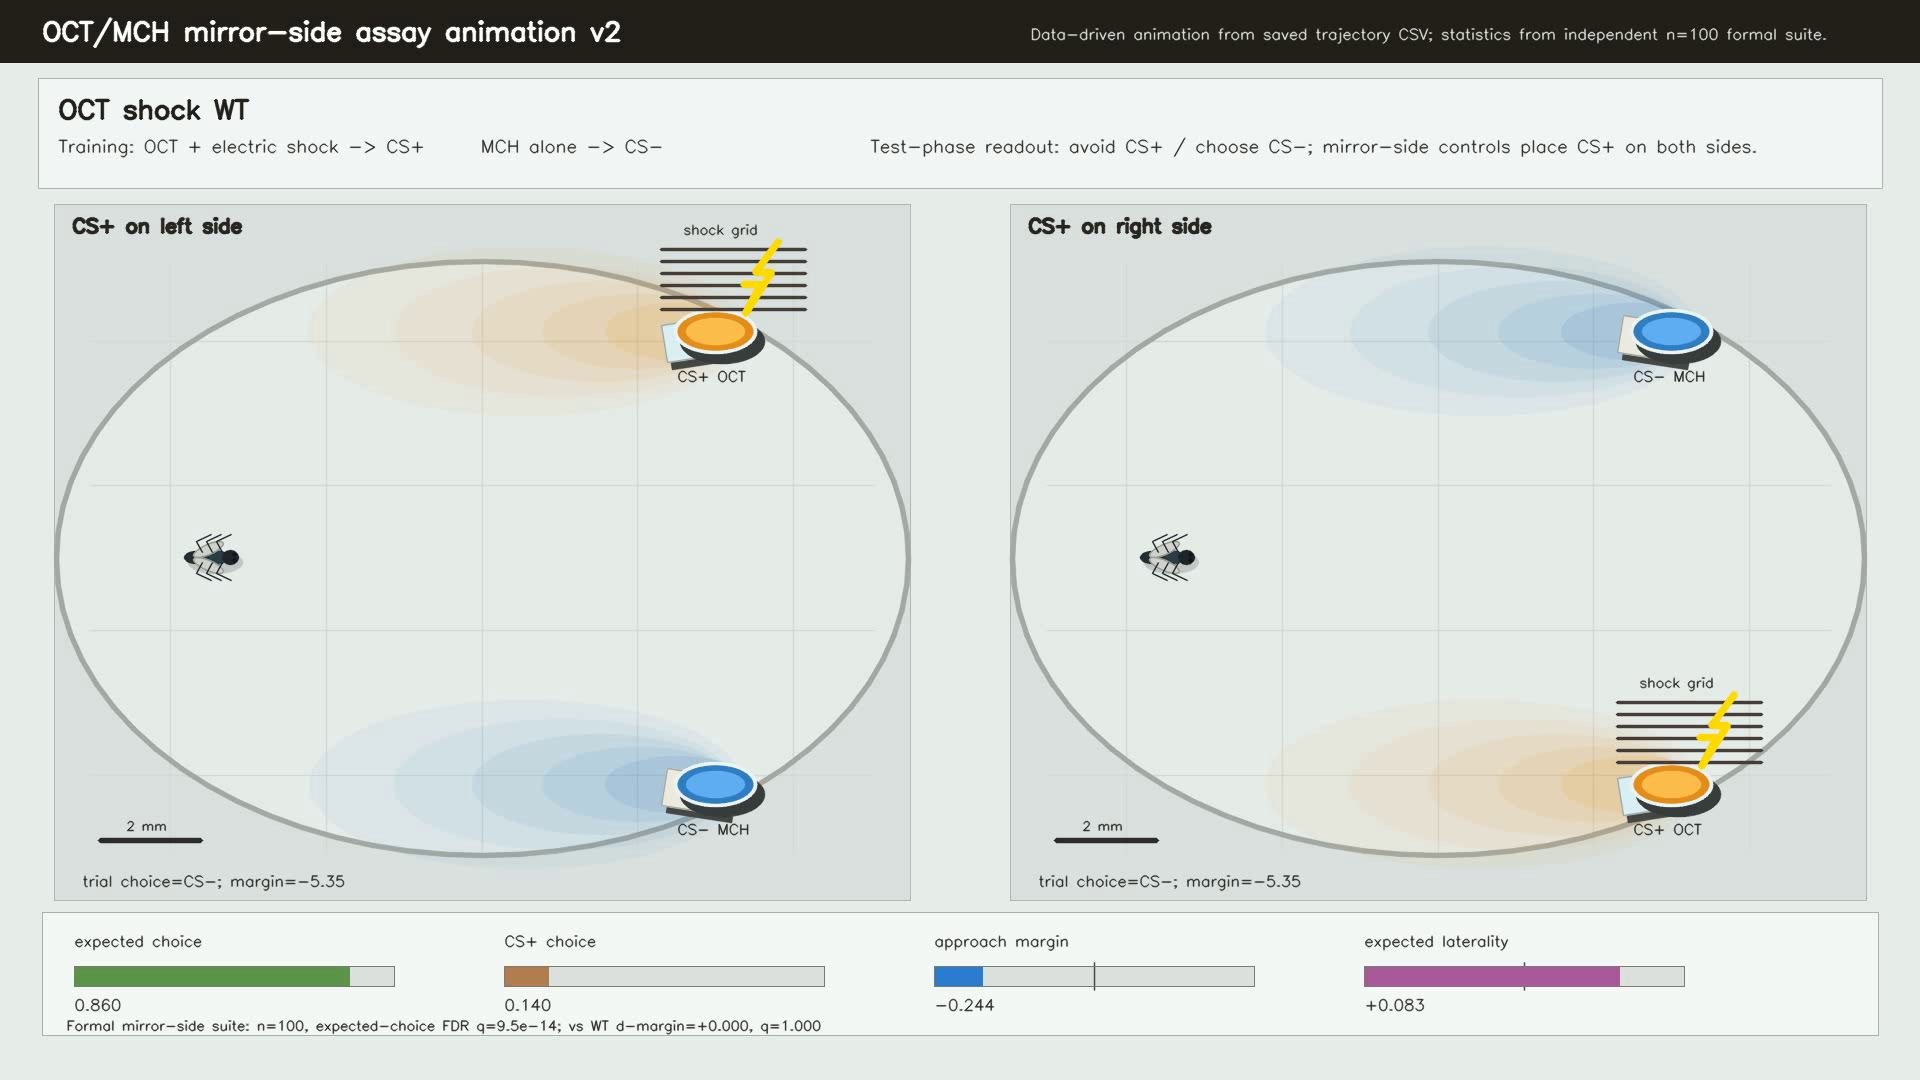
\includegraphics[width=\textwidth]{Fig_oct_mch_assay_v2_key_conditions_frame.png}
  \end{column}
  \begin{column}{0.33\textwidth}
    \begin{block}{视频中新增元素}
      \begin{itemize}
        \item 培养皿和实验边界。
        \item OCT/MCH 气味杯和气味羽流。
        \item 糖奖励和电击栅格。
        \item 果蝇朝向、轨迹尾迹、统计 inset。
      \end{itemize}
    \end{block}
    \begin{alertblock}{汇报口径}
      视频用于展示实验条件和轨迹，不替代统计检验。
    \end{alertblock}
  \end{column}
\end{columns}
\end{frame}

\begin{frame}{最重要的负结果：MB 扰动行为层还不够强}
\scriptsize
\begin{tabularx}{\textwidth}{@{}lrrrrX@{}}
\toprule
\textbf{扰动条件} & \textbf{n} & \textbf{选择率} & \textbf{$\Delta$margin} & \textbf{q} & \textbf{解释} \\
\midrule
left MB silenced & 100 & 0.89 & +0.032 & 1.0 & 与 WT 相比没有显著降低接近。\\
right MB silenced & 100 & 0.89 & +0.039 & 1.0 & 与 WT 相比没有显著改变选择。\\
MB symmetrized & 100 & 0.89 & +0.027 & 1.0 & 对称化没有产生预期行为下降。\\
MB swapped & 100 & 0.87 & -0.002 & 1.0 & 左右交换没有显著反转行为。\\
\bottomrule
\end{tabularx}
\vspace{0.6em}
\begin{alertblock}{这页必须主动讲}
当前系统支持“结构侧化可传播到功能读出”，但还不能严谨声称“MB 侧化已经改变真实果蝇行为”。这也是后续模型增强和湿实验验证的重点。
\end{alertblock}
\end{frame}

\begin{frame}{湿实验验证路径}
\small
\begin{columns}[T,onlytextwidth]
  \begin{column}{0.32\textwidth}
    \begin{block}{结构证明}
      GRASP / split-GFP 验证右侧 DPM/5-HT 到右侧 $\alpha'\beta'$ KC，以及左侧 Glu 到左侧 $\alpha'\beta'$ KC。
    \end{block}
  \end{column}
  \begin{column}{0.32\textwidth}
    \begin{block}{功能证明}
      DPM-driver 表达 CsChrimson/ReaChR；KC 或 MB compartment 表达 5-HT sensor / GCaMP；做 180 度旋转控制。
    \end{block}
  \end{column}
  \begin{column}{0.32\textwidth}
    \begin{block}{行为证明}
      独立群体做 OCT/MCH T-maze；重点测试 delayed/conflict 条件下红光 DPM stimulation 对 choice index 的改变。
    \end{block}
  \end{column}
\end{columns}
\vspace{0.4em}
\begin{center}
\blue{结构、功能、行为三条证据合在一起，才构成强论证。}
\end{center}
\end{frame}

\begin{frame}{当前风险}
\small
\begin{tabularx}{\textwidth}{@{}p{3.2cm}X@{}}
\toprule
\textbf{风险} & \textbf{处理方式} \\
\midrule
不是 Eon 私有闭环复刻 & 明确写成公开 surrogate，不声称连接组单独涌现完整行为。\\
NT 预测不是直接化学测量 & 需要 GRASP/split-GFP、5-HT sensor、GCaMP 或等价湿实验交叉验证。\\
行为代理对 MB 扰动不敏感 & 作为负结果保留；下一步增强 MBON/DAN/APL/DPM 到 DN 的在线控制接口。\\
OCT/MCH sensory encoder 简化 & 需要更细的 ORN/PN/glomerulus 到 KC 映射和真实气味浓度标定。\\
单只成像不能继续行为 & 成像和群体行为分开验证，用统计方向闭合证据链。\\
\bottomrule
\end{tabularx}
\end{frame}

\begin{frame}{下一步计划}
\small
\begin{enumerate}
  \item \textbf{模型增强：} 把 MBON/DAN/APL/DPM readout 接入在线行为控制器，而不是只做后验行为映射。
  \item \textbf{扰动增强：} 做 dose response、degree-preserving random、matrix symmetrization、left-right swap。
  \item \textbf{数据增强：} 引入更真实的 OCT/MCH sensory encoder 和 DN-to-motor calibration。
  \item \textbf{湿实验优先级：} 先做 DPM 红光 release imaging，再做 group T-maze conflict assay。
  \item \textbf{论文叙事：} 主文强调“结构侧化 + 功能传播 + 可验证预测”，把完整行为因果作为待验证目标。
\end{enumerate}
\end{frame}

\begin{frame}{组会 take-home message}
\small
\begin{block}{发现}
果蝇蘑菇体 KC 输入存在稳定递质侧化：右侧更偏 5-HT，左侧更偏 Glu，最强在与记忆巩固相关的 $\alpha'\beta'$ 区。
\end{block}
\begin{block}{仿真价值}
赛博果蝇 surrogate 把结构发现推进到功能传播和实验设计：侧化 seed 能到达 memory readouts，DPM 光遗传和 OCT/MCH conflict assay 是优先验证路线。
\end{block}
\begin{alertblock}{边界}
当前还不能说连接组单独涌现完整行为，也不能说 MB 侧化已经被真实行为因果证明。下一步必须用 DPM 成像、GRASP/split-GFP 和群体行为完成闭环。
\end{alertblock}
\end{frame}

\end{document}
